
\documentclass[11pt,a4wide]{article}
\usepackage{verbatim}
\usepackage{listings}
\usepackage{graphicx}
\usepackage{a4wide}
\usepackage{color}
\usepackage{amsmath}
\usepackage{amssymb}
\usepackage[dvips]{epsfig}
\usepackage[T1]{fontenc}
\usepackage{cite} % [2,3,4] --> [2--4]
\usepackage{shadow}
\usepackage{hyperref}
\usepackage{physics}

\setcounter{tocdepth}{2}

\lstset{language=c++}
\lstset{alsolanguage=[90]Fortran}
\lstset{basicstyle=\small}
\lstset{backgroundcolor=\color{white}}
\lstset{frame=single}
\lstset{stringstyle=\ttfamily}
\lstset{keywordstyle=\color{red}\bfseries}
\lstset{commentstyle=\itshape\color{blue}}
\lstset{showspaces=false}
\lstset{showstringspaces=false}
\lstset{showtabs=false}
\lstset{breaklines}

\title{ Project 1 in FYS-3150 }
\author{Gullik Vetvik Killie }

\begin{document}

\maketitle

\tableofcontents

\newpage

All the programs are in the gihub folder git@github.com:Gullik/Fys3150Gullik.git.

\section{Task a: Implement the Jacobi method to solve eigenvalue problems}
	\subsection{Theory behind the Jacobi method}
	The Jacobi method is an iterative method to make an approximated diagonal
	matrix in an eigenvalue problem by multiplying it several times with
	a rotational matrix, \(\mathbf{S}\), that is chosen so it sets some off diagonal 
	elements to \(0\). When multiplying it with the rotational matrix some of the already
	0 elements may get a nonzero value, so by always choosing the largest off-diagonal
	element hopefully it will produce a near diagonal end matrix. By also doing the rotation transformation 
	on the right and side the equation will be equal on both sides throughout and we can extract the eiganvalues
	easily at the end.
	
	\begin{align}
		\mathbf{A} \va{x} &= \lambda \va{x} 
		\\
		\intertext{Doing a transformation with the rotation matrix \(\mathbf{S} = 
		\begin{pmatrix}
		1 & &  &  \\
		 &  \ddots & & & \mbox{\huge 0} &  \\ \\
		 & & &\cos{\theta} & \cdots & -\sin{\theta} \\
		 & \mbox{\huge 0} &	& \vdots 	& 1 & \vdots \\
		 & &	& \sin{\theta} & \cdots & \cos{\theta}
		\end{pmatrix}
		\), in which we choose \(\theta\) so the wanted elements in \(\mathbf{A}\) becomes \(0\) }
		\mathbf{SA } \va{x} & = \lambda \mathbf{S}\va{x} \\
		\mathbf{SA(S^{-1}S)}\va{x} & = \lambda \mathbf{S} \va{x}
		\intertext{Then we introduce a new vector \(\va{y} = \mathbf{S} \va{x}\) and a new matrix \(\mathbf{B}=\mathbf{SAS^{-1}}\),
		 where  \(\mathbf{B}\) is more diagonal than \(\mathbf{A}\)}
		 \mathbf{B}\va{y} = \lambda \va{y}
	\end{align}
	
	\noindent We do this again untill desired level of diagonality of the matrix is achieved
	
	\subsection{The Jacobi method computationally}
		Since the matrix inversion \url{<http://en.wikibooks.org/wiki/LaTeX/Hyperlinks#.5Chyperref>} and multiplication \(O(n^3)\) (\url{<http://www.ee.ucla.edu/ee236b/lectures/num-lin-alg.pdf>}) (Put in proper references later bibtex) used in the Jacobi method is unecessarily heavy for the sparse
		rotational matrix \(\mathbf{S}\) we used a quicker method to do it.\\
		
		For a simplified \(3\cross3\) symmetric system the transformation \(\mathbf{B}=\mathbf{SAS^{-1}}\) becomes:
		
		\begin{align}
		\mathbf{B} &=
			\begin{pmatrix}
			1 & 0 & 0\\
			0 & c & -s\\
			0 & s & c
			\end{pmatrix}
			\begin{pmatrix}
			a_{11} & a_{12} & a_{13}\\
			a_{12} & a_{22} & a_{23}\\
			a_{13} & a_{23} & a_{33}
			\end{pmatrix}
			\begin{pmatrix}
			1 & 0 & 0\\
			0 & c & s\\
			0 & -s & c
			\end{pmatrix}
		\intertext{where \(c = \cos{\theta}, s = \sin{\theta}\)}
		\\
		&= 
			\begin{pmatrix}
			a_{11} 	&  	a_{12} & a_{13}
			\\
			c a_{12} - s a_{13}	& c a_{22} - s a_{23} & c a_{23} - s a_{33}
			\\
			sa_{12} + c a_{13} & sa_{22} + c a_{23} & sa_{23} + c a_{33}
			\end{pmatrix}
			\begin{pmatrix}
			1 & 0 & 0\\
			0 & c & s\\
			0 & -s & c
			\end{pmatrix}
		\\ &=
			\begin{pmatrix}
			a_{11} & c(a_{12}) - s(a_{13})	& s(a_{12}) + c(a_{13})
			\\
			c a_{12} - s a_{13}	& c(c a_{22} - s a_{23}) - s(c a_{23} - s a_{33})	& s(c a_{22} - s a_{23}) + c(c a_{23} - s a_{33})
			\\
			sa_{12} + c a_{13}	& c(sa_{22} + c a_{23}) - s(sa_{23} + c a_{33})	& s(sa_{22} + c a_{23}) + c(sa_{23} + c a_{33})
			\end{pmatrix}
		\\&=
			\begin{pmatrix}
			a_{11} & ca_{12} - sa_{13}	& sa_{12} + ca_{13}
			\\
			c a_{12} - s a_{13} 	& c^2a_{22} + s^2 a_33 -2sc a_{23}	& a_{23}(c^2 - s^2) + sc(a_{22}-a_{33})
			\\
			sa_{12} + c a_{13} 	& a_{23}(c^2 - s^2) + sc(a_{22} -a_{33})	& s^2a_{22} + c^2 a_{33} + 2 sca_{23}
			\end{pmatrix}
		\intertext{Then we choose \(\theta\) so that \(B_{23}=0\)}
		\mathbf{B} &= \begin{pmatrix}
			a_{11} & ca_{12} - sa_{13}	& sa_{12} + ca_{13}
			\\
			c a_{12} - s a_{13} 	& c^2a_{22} + s^2 a_33 -2sc a_{23}	& 0
			\\
			sa_{12} + c a_{13} 	& 0	& s^2a_{22} + c^2 a_{33} + 2 sca_{23}
			\end{pmatrix}
		\end{align}
		\noindent All the components of \(\mathbf{B}\) is now known so they can be calculated straightforward for \(\theta\).
		If we precalculate \(\cos{\theta}\) and \(\sin{\theta}\) the flops needed to calculate \(\mathbf{B}\) will be:
		
		\begin{itemize}
		\item First row: 4 multiplications and 2 additions
		\item Second row: 10 multiplications and 3 additions
		\item Third row: 10 multiplications and 3 additions
		\end{itemize}
		
		For a larger matrix we can ignore the all of the order \(O(N)\) operations since the higher order operations will overshadow them.
		The Jacobi rotation first finds the largest offdiagonal element, a \(\frac{N^2}{2} - N\) set of operations since it only need to 
		search through the upper half of the matrix since it is symmetric and it can ignore the diagonal. Doing the symmetry transformation
		it requires first \(O(N)\) order of operations to find the angle. To do the requires changes in the matrix it needs to go through 
		all the rows in the matrix and do four floating points operations and relocation. \(\sum_i^N(B_{ij})\) where four of the elements
		are changed for each row. The first change \(B_{ik} = cos(\theta)A_{ik} - \sin{\theta}A_{il}\) requires 2 multiplications and a subtraction,
		and the same for \(B_{il} = cos(\theta)A_{il} - \sin{\theta}A_{ik}\). It is symmetrical so we can use those changes again so we need
		\(6N\) floating points operations for each row, totaling up to \(6N^2\) FLOPS for the symmetry transformation. The whole Jacobi method 
		transformation with the finding of the largest off diagonal element totals appriximately \((6+\frac{1}{2})N^2\) FLOPS.
		\\ \\
		My implementation of the Jacobi method is in the github folder git@github.com:Gullik/Fys3150Gullik.git and is 
		contained in the file JacobiRot.cpp. It works by calling the JacobiRot() function and it then subsequently finds the 
		largest offdiagonal element by the function MaxOffDiag(), and then does the rotation by the Rotation function.

\section{Task b: Playing with the Jacobi algorithm on the Harmonic oscillator}
	\subsection{Steps vs well edge} 
	The number of steps, \(N\), decides the and how finegrained our approximation of the 3D potential well is.
	 \(\rho_{max} \)is also important for how good the approximation becomes, since the wave function is supposed to approach
	 0 at infinity distance away and at \(0\), and \(\rho_{max}\) is where we define that infinity to be. Since the potential is decreasing by \(r^2\)(?)
	 it is decreasing quite fast and \(\rho_{max} \) does not need to be very large for it to cover most of the wavefunction.
	 Unfortunately as we increase the area we cover by letting \(\rho_{max} \) grow, we need more steps, \(N\) to be able to cover
	 the area inbetween to good enough detail and a large N slows down the Jacobi algorithm to a great extent. 
	 In table \ref{table:Steps} (Reference numbering wrong) the needed number of steps needed to achieve 4 signaficant figures correct
	  on the first three eigenvalues of a three dimensional harmonic oscillator, \(\lambda_n = 3, 7 , 11 , ...\).
	
	\begin{table}
		\begin{tabular}{|r|l|l|l|l|l|}
		\hline 
		\(\mathbf{\rho_{max}}\) 	& 1 	& 2.5	& 5	  &		10	&	2
		\\
		\hline
		\textbf{N} 					& - 	& 	-	& 175 &		- 	&	2	
		\\ \hline
		\end{tabular}
	\label{table:Steps}
	\caption{The steps needed to get 4 signficant figures on the first three eignvalues for different values of \(\rho_{max}\)}
	\end{table}
	
	\subsection{Comparing it with the solver from the armadillo library}
	\begin{table}
		\begin{tabular}{|c|l|l|l|l|l|}
		\hline
		N			& 	10			&	50			&	100			&	500			&	1000
		\\ \hline
		eig\_sym	&	1.25e-4s	&	0.001431s	&	0.004766s	&	0.17468s	&	1.07868s
		\\	\hline		
		Jacobi\_Rot	&	4.3e-5s		&	0.019119s	&	0.349412s	&	352.13s		&	8702.44s
		\\ \hline
		Rotations	& 13			&	856			& 	6483		& 	265300		&	1123182
		\\ \hline
		\end{tabular}
	\caption{The time test where done with \(\rho_{max}= 20\) and a tolerance of \( \epsilon = 0.001\), value of \(\rho_{max}\) 
			decides the sparseness of the matrix, while \(\epsilon\) decides the accuracy. With the chosen tolerance the eigenvalues 
			agreed with the ones from the Armadillo solver for \(6\) significant figures for most configurations.
			Rotations is the number of applications of the symmetric transform that was applied by the Jacobi\_Rot before the offdiagonal elements was below 
			the tolerance \(\epsilon\)}
	\end{table}
	
	The function when tested got the wanted results of the first three eigenvalues \(\lambda_i = 3, 7, 11\).
	
\section{Task c: The groundstate of two electrons in a harmonic potetial well}
	\subsection{Theory}
		Let us first start with a standard equation for two noninteracting particles in a potential well
		
		\begin{align}
		\left(  -\frac{\hbar^2}{2 m} \frac{d^2}{dr_1^2} -\frac{\hbar^2}{2 m} \frac{d^2}{dr_2^2}+ 
		\frac{1}{2}k r_1^2+ \frac{1}{2}k r_2^2\right)u(r_1,r_2)  &= E^{(2)} u(r_1,r_2)
		\intertext{We introduce a a new coordinate between the particles, \(\vec{r} = \vec{r_1} -\vec{r_2}\) 
		and a center of mass coordinate coordinate \(\vec{R} = \frac{\vec{r_1} +\vec{r_2}}{2}\)}
		\left(  -\frac{\hbar^2}{m} \frac{d^2}{dr^2} -\frac{\hbar^2}{4 m} \frac{d^2}{dR^2}+ \frac{1}{4} k r^2+  kR^2\right)u(r,R)
		  &= E^{(2)} u(r,R)
		\intertext{The energy can be seperated into a center of mass and a relative energy, we will only focus on the relative energy. 
		Adding the repulsion between them the radial equation becomes:}
		\left(  -\frac{\hbar^2}{m} \frac{d^2}{dr^2}+ \frac{1}{4}k r^2+\frac{\beta e^2}{r}\right)\psi(r)  &= E_r \psi(r) 
		\\
		\intertext{Introducing a dimensionless variabe \(\rho = \frac{r}{\alpha}\) and choosing \(\alpha = \frac{\hbar^2}{m\beta e^2}\) the radial equation becomes} 
		-\frac{d^2}{d\rho^2} \psi(\rho) + \omega_r^2\rho^2\psi(\rho) +\frac{1}{\rho}\psi(\rho) &= \lambda \psi(\rho)
		\end{align}
	\noindent This will be discretized in the same way as in task b, except that the diagonal becomes 
	\(d_i = -\frac{1}{h^2} + \omega_r^2(\rho_{min} + ih)^2\), where \(h\) is the stepsize.
	
	\subsection{Analysis}
		The computation is carried out with main.cpp in the github folder, by choosing task = 2. 
		
		We were not able to find any stable eigenvalues that did not depend upon the choice of \(\rho_{max}\) and \(N\). 
		We could also not get it to produce the wanted values found in (M.Taut, Physical Review A, 1993) which should give eigenvalues
		of \(0.625\) for \(\omega_r = 1/4\). The eigenvalues where stable for \(\omega_r = 0.5, 1 \text{ and } 5 \) and are given in 
		table \ref{table:Oscillator_pot}. The eigenvalues grew stronger as the oscillator potential grew stronger, which indicates that the 
		electrons where forced closer together.
		
		\begin{table}
			\begin{tabular}{c || l | l | l}
			\hline
			\(\omega_r\) &	\(\lambda_1\) & \(\lambda_2\) & \(\lambda_3\)
			\\ \hline
			0.5			&	2.2		&		4.1			&	6.0
			\\ \hline
			1.0			&	4.1		&		7.9			&	11
			\\ \hline	
			5.0 		&	17		&		37		&	56
			\end{tabular}
			\caption{Table over eigenvalues for different oscillator potentials. The eigenvalues, which are proportional to the 
			relative energy between them gets stronger as the oscillator potential grows stronger.}
			\label{table:Oscillator_pot}
		\end{table}

	\section{Task d: Plotting the eigenfunctions}
	
	The main.cpp function stores the eigenvectors as a csv file which is then plotted by a small python script, called Plots.py in the same github folder.
	\\ \\
	The results for the groundstates are plotted in figure \ref{fig:wavefunctions}, and shows how the electron clouds far apart the electron clouds tend to be.
	The results for the lowest oscilatore potential of \(\omega = 0.5\) is plotted in figure \ref{fig:0_5} and shows that the wavefunctions is not
	contained by the potential well for the exited states. In figures \ref{fig:1} and \ref{fig:5} the wavefunctions are shown for oscillator 
	potentials of \(1\) and \( 5\) and the two electrons are kept quite close by the well.  All of the wavefunctions are yet to be normalised.
	
	\begin{figure}
		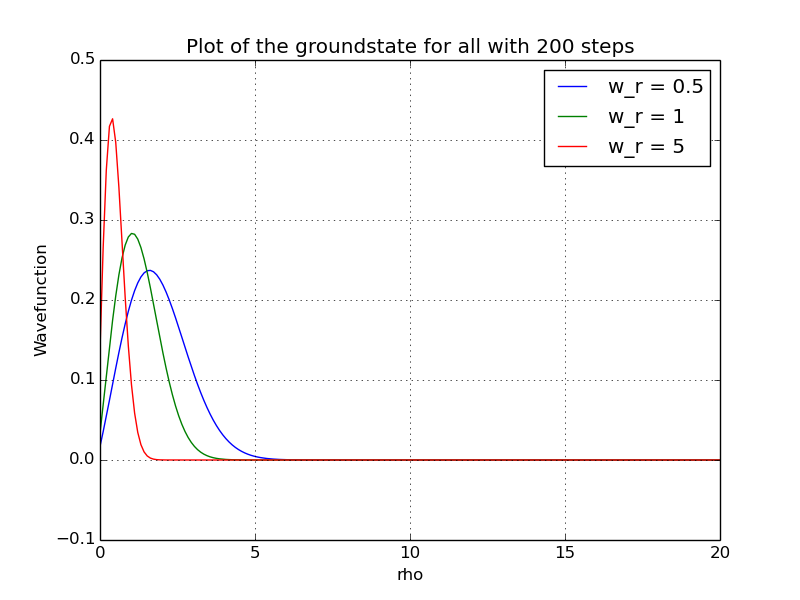
\includegraphics[scale = 0.5]{/home/gullik/Documents/Fys3150Gullik/Project_2/Project_2_Gullik/Plot of the groundstate with200.png}
		\label{fig:wavefunctions}
		\caption{A plot of the different functions for the relative distance between two electrons in a three dimensional harmonic potential well.
		Both the electrons are in their ground state. When the oscillator potential is strong the electrons, stay relatively close as the oscillator
		potential forces them together}
	\end{figure}
	
	\begin{figure}
		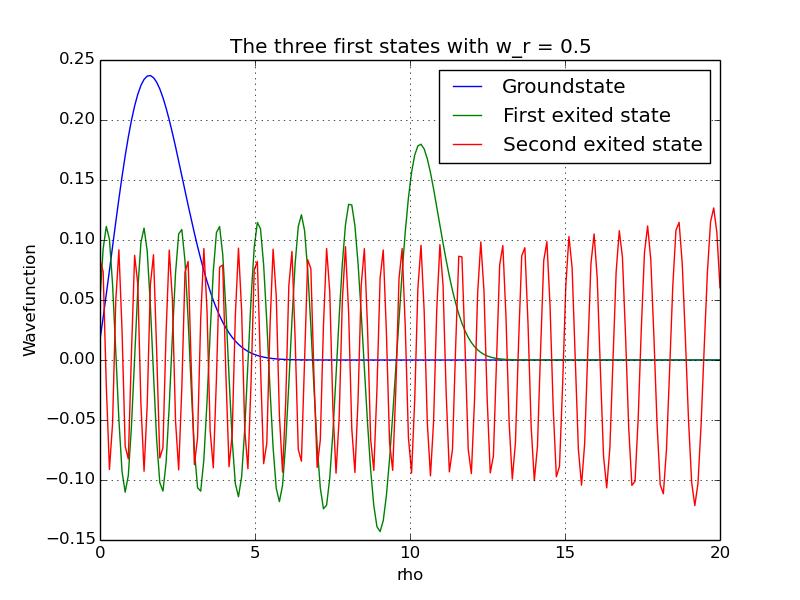
\includegraphics[scale = 0.5]{/home/gullik/Documents/Fys3150Gullik/Project_2/Project_2_Gullik/3stateswr05.png}
		\caption{The first three states of the relative distance between the two electrons with an oscillator potential of 0.5. 
		Both the exited states have enough energy to not be contained by the potential well}
		\label{fig:0_5}
	\end{figure}
	
	\begin{figure}
		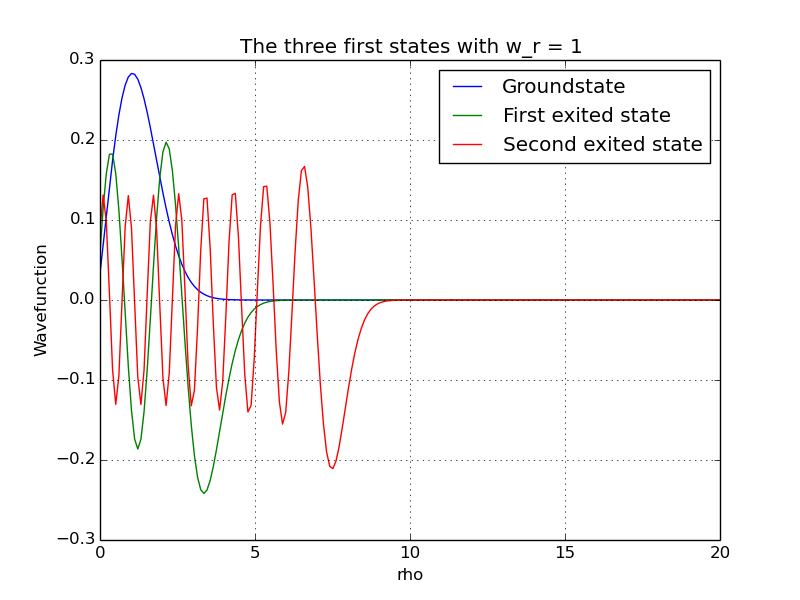
\includegraphics[scale = 0.5]{/home/gullik/Documents/Fys3150Gullik/Project_2/Project_2_Gullik/3stateswr1.png}
		\caption{The first three states of the relative distance between the two electrons with an oscillator potential of 1. 
		The electrons are bound for all the states}
		\label{fig:1}
	\end{figure}
	
	\begin{figure}
		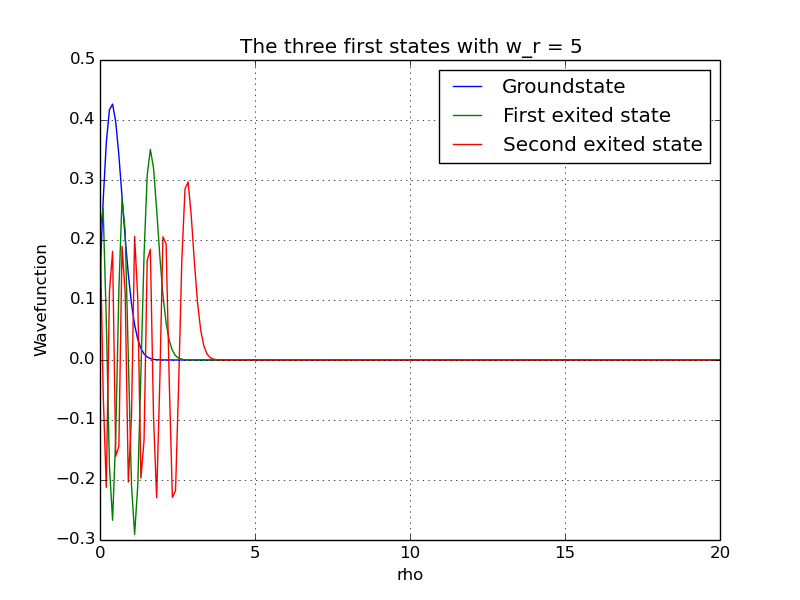
\includegraphics[scale = 0.5]{/home/gullik/Documents/Fys3150Gullik/Project_2/Project_2_Gullik/3stateswr5.png}
		\caption{The first three states of the relative distance between the two electrons with an oscillator potential of 1. 
		The electrons are bound for all the states}
		\label{fig:5}
	\end{figure}



\end{document}
